%%\documentclass[sn-nature]{sn-jnl}% Style for submissions to Nature Portfolio journals
%%\documentclass[sn-basic]{sn-jnl}% Basic Springer Nature Reference Style/Chemistry Reference Style
\documentclass[sn-mathphys,Numbered]{sn-jnl}
\usepackage{graphicx}%
\usepackage{multirow}%
\usepackage{amsmath,amssymb,amsfonts}%
\usepackage{amsthm}%
\usepackage{mathrsfs}%
\usepackage[title]{appendix}%
\usepackage{xcolor}%
\usepackage{textcomp}%
\usepackage{manyfoot}%
\usepackage{booktabs}%
\usepackage{algorithm}%
\usepackage{algorithmicx}%
\usepackage{algpseudocode}%
\usepackage{listings}%
\usepackage[normalem]{ulem}

% Make Orcid icon
\newcommand{\orcidicon}{
\includegraphics[width=0.32cm]{orcid.pdf}}
\newcommand{\orc}[1]{\href{https://orcid.org/#1}{\orcidicon}}

% Author Orcid ID: Define per author
\newcommand{\orcA}{0000-0001-8217-1484}
\newcommand{\orcB}{0000-0001-5038-8427}
\newcommand{\orcC}{0000-0001-5474-2649}
\newcommand{\orcD}{0000-0003-2704-6474}

% List of useful macros
\newcommand{\req}[1]{Eq.~(\ref{#1})}
\newcommand{\rf}[1]{Fig.~{\ref{#1}}}
\newcommand{\rt}[1]{Table~{\ref{#1}}}
\newcommand{\rsec}[1]{Sec.~{\ref{#1}}}
\newcommand*{\TeV}{\text{ TeV}}
\newcommand*{\GeV}{\text{ GeV}}
\newcommand*{\MeV}{\text{ MeV}}
\newcommand*{\keV}{\text{ keV}}
\newcommand*{\eV}{\text{ eV}}
\newcommand*{\meV}{\text{ meV}}
\DeclareMathOperator{\sgn}{sgn}

% Useful macros for annotation
\newcommand*{\xred}{\color{red}}
\newcommand*{\xblue}{\color{blue}}
\newcommand*{\xgreen}{\color{green}}
\newcommand*{\xmagenta}{\color{magenta}}
\newcommand{\rev}[1]{{\color{blue}#1}}
\newcommand*{\rcite}{{\xred (Citation?)}}

%\theoremstyle{thmstyleone}%
%\newtheorem{theorem}{Theorem}
%\newtheorem{proposition}[theorem]{Proposition}% 
%\theoremstyle{thmstyletwo}%
%\newtheorem{example}{Example}%
%\newtheorem{remark}{Remark}%
%\theoremstyle{thmstylethree}%
%\newtheorem{definition}{Definition}%

\raggedbottom
\begin{document}

%\title[Article Title]{Cold Ideal Fermi Gas}
\title[Article Title]{Decomposition of Fermi gas into zero and finite temperature components with examples}

%%=============================================================%%
%% Prefix	-> \pfx{Dr}
%% GivenName	-> \fnm{Joergen W.}
%% Particle	-> \spfx{van der} -> surname prefix
%% FamilyName	-> \sur{Ploeg}
%% Suffix	-> \sfx{IV}
%% NatureName	-> \tanm{Poet Laureate} -> Title after name
%% Degrees	-> \dgr{MSc, PhD}
%% \author*[1,2]{\pfx{Dr} \fnm{Joergen W.} \spfx{van der} \sur{Ploeg} \sfx{IV} \tanm{Poet Laureate} 
%%                 \dgr{MSc, PhD}}\email{iauthor@gmail.com}
%%=============================================================%%

\author[1]{\fnm{Cheng Tao} \sur{Yang\orc{\orcB}}}
\author[1,2]{\fnm{Martin} \sur{Formanek\orc{\orcD}}}
\author[1]{\fnm{Andrew} \sur{Steinmetz\orc{\orcC}}} 
\author[1]{\fnm{Johann} \sur{Rafelski\orc{\orcA}}}
%\email{iiiauthor@gmail.com}
%\equalcont{These authors contributed equally to this work.}

\affil[1]{\orgdiv{Department of Physics}, \orgname{The University of Arizona}, \city{Tucson}, \state{Arizona}, \postcode{85721}, \country{USA}}

\affil[2]{\orgdiv{ELI Beamlines Facility}, \orgname{The Extreme Light Infrastructure ERIC}, \orgaddress{ \postcode{252 41}, \city{Dolni Brezany}, \country{Czech Republic}}}

\abstract{The most interesting physics of finite temperature Fermi gasses occurs around the Fermi surface, which needs a mathematical tool that can capture the finite temperature behavior of the Fermi-Dirac distribution in an analytic fashion. We provide a novel form of the Fermi distribution that can separate the Fermi gas into zero and finite temperature components analytically which is useful for addressing physics beyond the zero temperature approximation.}


\date{To be published in International Journal of Theoretical Physics}
\keywords{Fermi distribution, Low temperature Fermi gas}

%%\pacs[JEL Classification]{D8, H51}
%%\pacs[MSC Classification]{35A01, 65L10, 65L12, 65L20, 65L70}

\maketitle

%%%%%%%%%%%%%%%%%%%%%%%%%%%%%%%%%%%%%%%
\section{Introduction}
\label{sec1}
%%%%%%%%%%%%%%%%%%%%%%%%%%%%%%%%%%%%%%%
Systems which obey the Fermi-Dirac (FD) distribution, such as finite temperature Fermi quantum gasses, are difficult to study outside the zero temperature limit because the numerical precision of finite temperature contribution rapidly vanishes\rcite. Numerical evaluations of the finite temperature behavior of systems also obscures the physics as the precise origin of thermodynamic features are shrouded; whereas analytic evaluations can show explicitly the mathematical origin of physical features. This is why the few analytic solutions that exist in physics are invaluable to study.

% Kapusta and Gale - many body theory
% Lebellac - text
% 

The most interesting physics of Fermi gasses occurs at finite temperatures~\cite{Elze:1980er} which necessitates a mathematical tool which captures the finite temperature behavior of the FD distribution in an analytic fashion. We provide a novel form of FD distribution that can separate the Fermi gas into zero and finite temperature components analytically which is useful addressing physics beyond the zero temperature approximation. We also tackle the case of the magnetized relativistic Fermi gas to demonstrate the usefulness of this new method. Other use cases would be for compact astrophysical systems (white dwarfs, neutron stars, quark stars)~\cite{Kaspi:2017fwg,Ferrer:2019xlr,Ferrer:2023pgq}, Early Universe phenomenology~\cite{Rafelski:2021aey,Rafelski:2023emw,Grayson:2023flr,Steinmetz:2023nsc}, quark-gluon plasmas (QGP)~\cite{Letessier:2002ony,Rafelski:2020ajx,Yang:2021bko}, and wherever finite temperature Fermi effects are important.

Before we introduce the novel form in \rsec{NewFermi}, we will briefly recall the standard picture of the FD distribution. In the zero temperature limit $T\to0$, the FD distribution reduces to a step function where a state $E_{i}$ is either filled or empty. For given chemical potential $\widetilde\mu(T)$, we have
\begin{align}
\label{f_old}
f_\mathrm{FD}(E_{i},\widetilde\mu(T),T)=\left[\exp\left(\frac{E_{i}-\widetilde\mu}{T}\right)+1\right]^{-1}\,,\quad
\lim_{T\to0}f_\mathrm{FD}=\left\{
\begin{array}{c}
1,\quad\mathrm{for}\quad{E_{i}}<\widetilde\mu\\
0,\quad\mathrm{for}\quad{E_{i}}>\widetilde\mu
\end{array}
\right.\,.
\end{align}
The energy of the last filled state is called the Fermi energy and is denoted by $E_F$. The Fermi energy is also the value of the chemical potential at zero temperature $T=0$, \emph{i.e.} $E_F\equiv\widetilde\mu(T = 0)$.

%%%%%%%%%%%%%%%%%%%%%%%%%%%%%%%%%%%%%%%
\begin{figure}[ht]
\centering
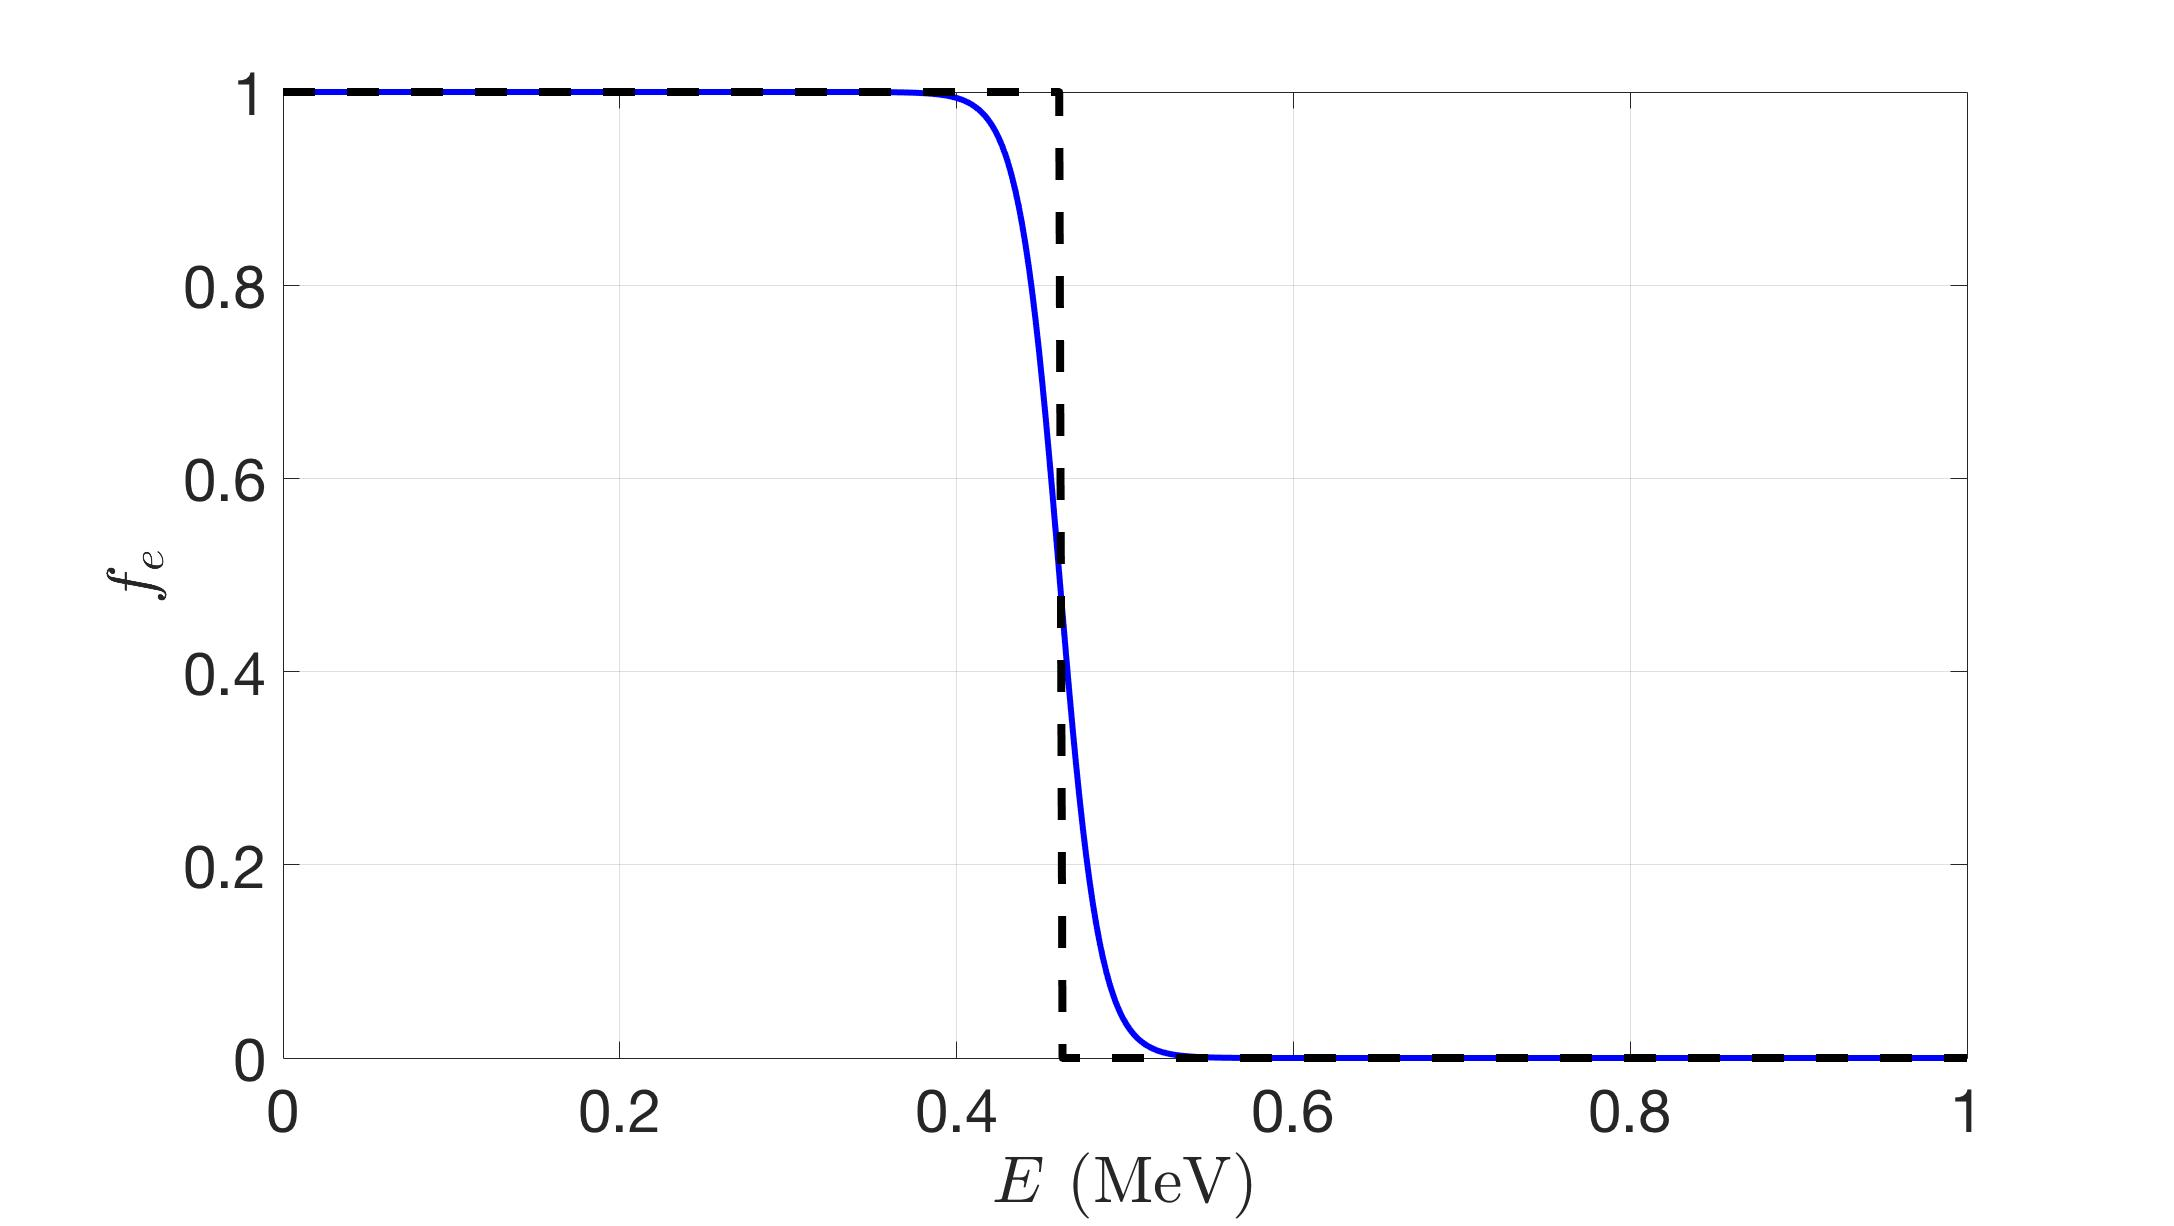
\includegraphics[width=0.9\textwidth]{./plot/Electron_distribution001}
\caption{The FD distribution is plotted (solid blue line) as a function of energy with parameters $T=0.012\MeV$ and $\widetilde\mu=0.461\MeV$. The zero temperature distribution is plotted as the dashed black line.}
\label{Electron_001}
\end{figure}
%%%%%%%%%%%%%%%%%%%%%%%%%%%%%%%%%%%%%%%

In \rf{Electron_001} we plot the FD distribution of a fermion as a function of energy with example parameters $T=0.012\MeV$ and $\widetilde\mu=0.461\MeV$. This shows the textbook behavior that for finite temperatures, there is a filling of higher energy states above the chemical potential $\widetilde\mu$ at the expense of states below $\widetilde\mu$. As the temperature increases, the distribution becomes more broad as a wide range of states become thermally populated.

%%%%%%%%%%%%%%%%%%%%%%%%%%%%%%%%%%%%%%%
\section{Zero and finite temperature Fermi-Dirac distributions}
\label{NewFermi}
%%%%%%%%%%%%%%%%%%%%%%%%%%%%%%%%%%%%%%%
\subsection{A novel form of Fermi-Dirac distribution}
\label{Novel}
%%%%%%%%%%%%%%%%%%%%%%%%%%%%%%%%%%%%%%%
Our interest and motivations in studying the Fermi-Dirac distribution was to perform cosmological computations involving both high and low temperature physics. In doing so, we have identified the following novel way to write FD distribution as three terms which separates out the zero temperature portion from the finite temperature contributions as 
\begin{align}
\label{NFF1}
\begin{split}
f_\mathrm{FD}(x)
&=\left(e^{x}+1\right)^{-1}\\
&=\Theta(-x)+\frac{1}{2}e^{-|x|}\left[\sgn(x)+\tanh(x/2)\right]\,,\quad
x\equiv\frac{E-\widetilde\mu}{T}\,,
\end{split}
\end{align}
\begin{align}
\label{NFF2}
\Theta(x)=\left\{
\begin{array}{r}
1,\quad\mathrm{for}\quad{x}>0\\
1/2,\quad\mathrm{for}\quad{x}=0\\
0,\quad\mathrm{for}\quad{x}<0
\end{array}\right.\,,\qquad
\sgn(x)=\left\{
\begin{array}{r}
+1,\quad\mathrm{for}\quad{x}>0\\
0,\quad\mathrm{for}\quad{x}=0\\
-1,\quad\mathrm{for}\quad{x}<0\\
\end{array}\right.\,,
\end{align}
where $\Theta(x)$ is the Heaviside step function and $\sgn(x)$ is the sign function. The first term $\Theta(-x)$ in \req{NFF1} represents the zero temperature portion of the FD distribution while the finite temperature terms are weighted by a decaying exponential function. The immediate benefit of this form is that numerical evaluations will naturally center around the Fermi surface of the system with finite temperature contributions exponentially weighted.

We note that \req{NFF1} comprises of distributions rather than analytical functions~\cite{Arfken:2011abc}. On first sight, it is difficult to see that these cancel to create the analytical FD function seen in \req{f_old}. In the following section, we will show that both sides are truly equivalent.

%%%%%%%%%%%%%%%%%%%%%%%%%%%%%%%%%%%%%%%
\subsection{Mathematical proof}
\label{Proof}
%%%%%%%%%%%%%%%%%%%%%%%%%%%%%%%%%%%%%%%
To show the equivalency between the two distinct forms of the FD, we look at the three relevant regions of $x>0$, the origin $x=0$, and $x<0$. For $x>0$, \req{NFF1} evaluates as
\begin{equation}
    f_\mathrm{FD}(x>0) = 0 + \frac{1}{2}e^{-x}[1+\tanh(x/2)] = (e^x + 1)^{-1}\,.
\end{equation}
This can be seen by substituting
\begin{equation}
    \tanh(x/2)=\sinh(x/2)/\cosh(x/2)\,,
\end{equation}
and using hyperbolic formulas
\begin{equation}
    \sinh(x/2)=(e^{x/2}-e^{-x/2})/2\,,\qquad
    \cosh(x/2) = (e^{x/2}+e^{-x/2})/2\,.
\end{equation}
In a similar manner, the $x<0$ region evaluates as
\begin{equation}
    f_\mathrm{FD}(x<0) = 1 + \frac{1}{2}e^{x}[-1 + \tanh(x/2)] = (e^x + 1)^{-1}\,.
\end{equation}

As our expression is written in terms of distributions rather than analytic functions, special care should be taken in evaluation of the origin. It can be shown that the left $x=0^{-}$ and right $x=0^{+}$ limits are equal via
\begin{align}
    \lim_{x\rightarrow 0^+} f_\mathrm{FD}(x) &= 0 + \frac{1}{2}(1 + 0) = \frac{1}{2}\,,\\
    \lim_{x\rightarrow 0^-} f_\mathrm{FD}(x) &= 1 + \frac{1}{2}(-1 + 0) = \frac{1}{2}\,,
\end{align}
which means that the limit of our expression at the origin $x=0$ exists and is equal to the value of the function in \req{f_old} at $x = 0$. With the definitions of the step function $\Theta(x)$ and sign function $\sgn(x)$ in \req{NFF2}, the limits for $x\rightarrow0^{\pm}$ are equal to the value of our function at the origin. Therefore, for all real $x\in\mathbb{R}$, our expression matches the original FD distribution \req{f_old}.

\rev{This I believe is not necessary...if the functions match $\forall x \in \mathbb{R}$ then of course their derivatives match too - NOT TRUE FOR DISTRIBUTIONS!.}Lastly, we check that the properties of the first derivative of \req{NFF1} are in agreement with the usual FD distribution. We write the first derivative of the singular distributions as 
\begin{align}
\label{NFF1b}
\frac{d}{dx}\Theta(-x)&=-\delta(x)\,,\qquad 
\frac{d}{dE}\Theta(-x)=-\frac{1}{T}\delta(x)\,,\\
\frac{d}{dx}\sgn(x)&=2\delta(x)\,,\,\,\quad 
\frac{d}{dE}\sgn(x)=\frac{2}{T}\delta(x)\,,
\end{align}
both without and with units and where $\delta(x)$ is the Dirac $\delta$-function. These cancel in \req{NFF1} at $x=0$ exactly as required since the derivative of the FD distribution written in \req{f_old} lacks a $\delta$-function. This encourages us to believe that all of singular expressions cancel leaving it fully analytic. This completes our demonstration of the validity of \req{NFF1}.

%%%%%%%%%%%%%%%%%%%%%%%%%%%%%%%%%%%%%%%
\subsection{Decomposition of zero and finite temperature contribution}
\label{Numerical}
%%%%%%%%%%%%%%%%%%%%%%%%%%%%%%%%%%%%%%%
%\sout{In addition to our mathematical derivation, we also present a graphical check to show that the novel expression for the distribution is well behaved numerically. In \rf{Fermi_Checking} we plot the traditional expression for the Fermi-distribution [\req{f_old}] with solid lines and the novel form of Fermi-distribution [\req{NFF1}] with dashed lines as a function of energy for various temperatures and chemical potential values. This demonstrates that \req{f_old} and \req{NFF1} are equivalent to each other numerically.}\rev{I would remove this and Fig.2. ...of course they are identical, we showed that they are. Or I would at least reframe Fig. 2. as examples of Fermi distribution for some parameters, not sure if needed. This way it makes an impression that we are not sure. I would focus on the splitting in Fig. 3.}

%%%%%%%%%%%%%%%%%%%%%%%%%%%%%%%%%%%%%%%
%\begin{figure}[ht]
%\centering
%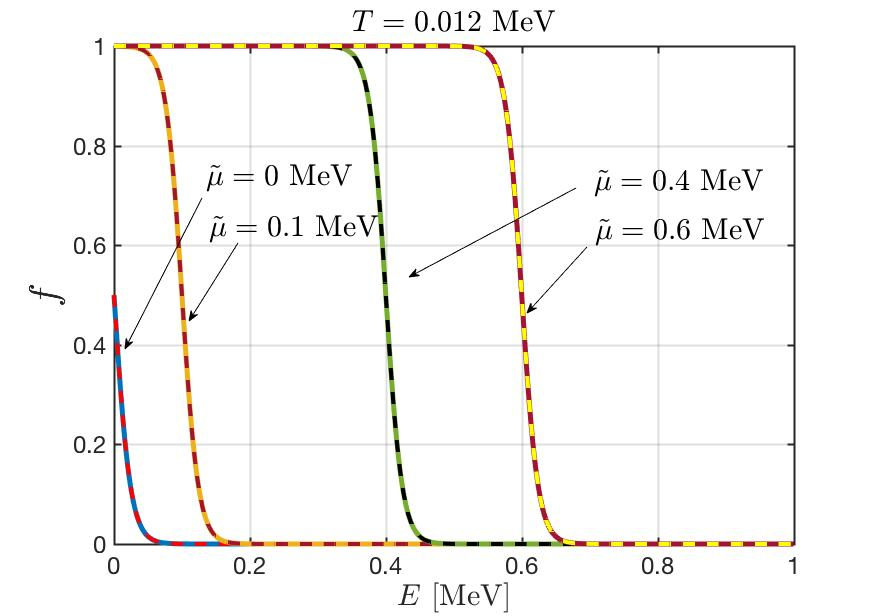
\includegraphics[width=0.5\textwidth]{./plot/Fermi_novel_001}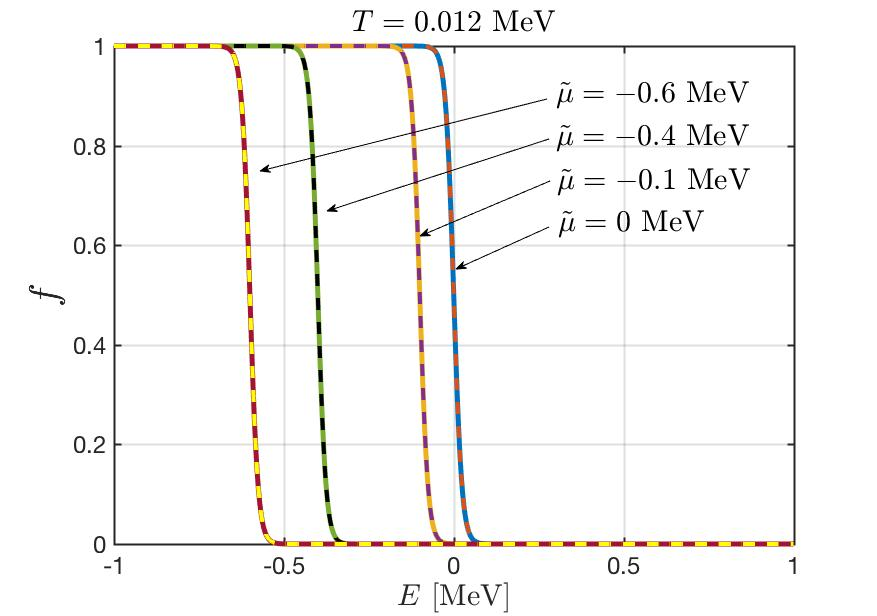
\includegraphics[width=0.5\textwidth]{./plot/Fermi_novel_002}
%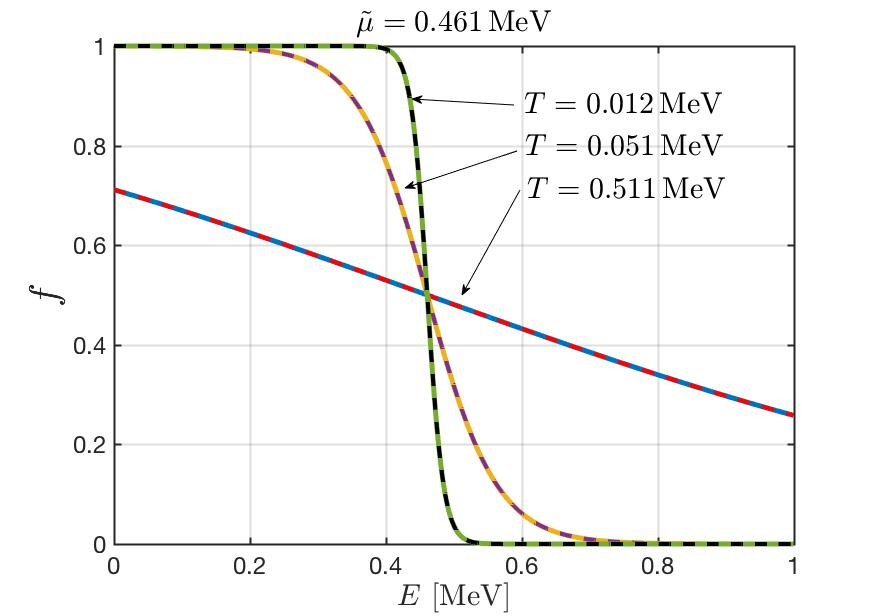
\includegraphics[width=0.5\textwidth]{./plot/Fermi_novel_003}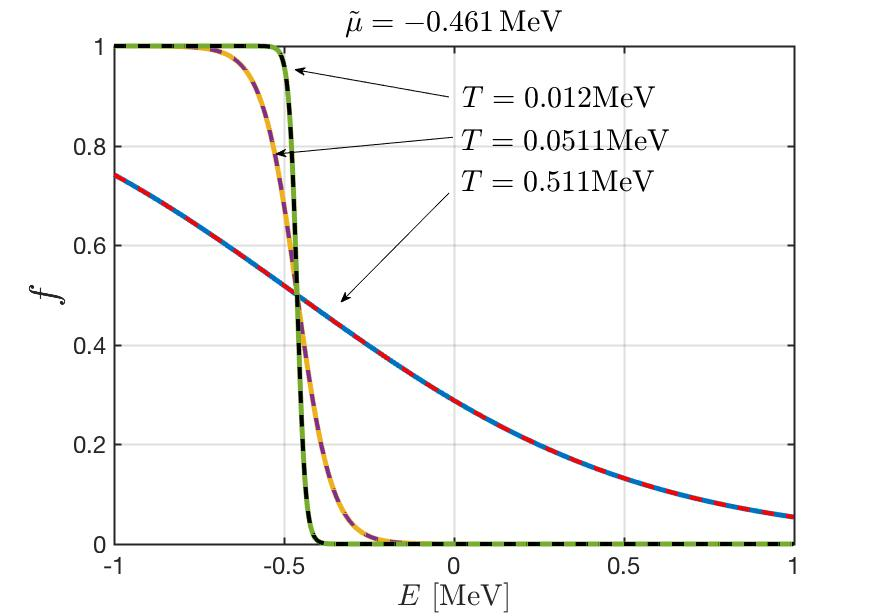
\includegraphics[width=0.5\textwidth]{./plot/Fermi_novel_004}
%\caption{We plot the Fermi-distribution~\req{f_old} (solid lines) against the novel formulation~\req{NFF1} (dashed lines) as a function of energy. (Upper plots) We compare the two formulations under different chemical potentials: $\widetilde\mu=(0,\pm0.1,\pm0.4,\pm0.6)\MeV$ at temperature $T=0.012\MeV$. (Lower plots) We compare under different temperatures $T=(0.511,0.0511, 0.012)\MeV$ for chemical potential $\widetilde\mu=\pm0.461\MeV$.}
%\label{Fermi_Checking}
%\end{figure}
%%%%%%%%%%%%%%%%%%%%%%%%%%%%%%%%%%%%%%%

%{\xmagenta ANDREW: I recommend we stick with the dimensionless variable ``$x$'' for all calculations and discussions up to the physical example. This enhances the mathematical clarity and simply makes the expressions more simple to read. I did this for Eq. 11, but wanted your approval before continuing my edits. Additionally, the expression $f_{T=0}(x)$ doesn't make sense as $T$ is clearly nonzero in $x(E,\widetilde\mu,T)$. I suggest we abandon this notation and simply call it the step function $\Theta(x)$ and we are already doing earlier. There is also a conflict where Eq. 12 and Eq. 13 are defined using the same notation. Is this an error? Please look at this Cheng Tao.} 
To illustrate the separation of the zero and finite temperature contributions to the FD distribution, it is convenient to rewrite Eq.~(\ref{NFF1}) in the following form
\begin{align}\label{Eq_form}
&f_\mathrm{FD}(x)=\Theta(-x)+f_\mathrm{T\neq0}(x)+\tilde f_\mathrm{T\neq0}(x)
\end{align}
where the temperature functions are defined as
\begin{align}
&f_\mathrm{T\neq0}=\frac{1}{2}e^{ -|x|/T }\mathrm{sgn}\left(x\right),\qquad
\tilde f_\mathrm{T\neq0}=\frac{1}{2}e^{ - |x| }\tanh\left(\frac{x}{2}\right),\qquad x=\frac{E-\tilde\mu}{T}
%&f_\mathrm{T\neq0}=\frac{1}{2}e^{ - |E-\widetilde\mu|/T }\mathrm{sgn}\left(\frac{E-\widetilde\mu}{T}\right),\qquad
%\tilde f_\mathrm{T\neq0}=\frac{1}{2}e^{ - |E-\widetilde\mu|/T }\tanh\left(\frac{E-\widetilde\mu}{2T}\right)
\end{align}
In Fig.~(\ref{Fermi_Component}) we plot the exact Fermi distribution (black line $f$), the zero (purple lines, $f_{T=0}$) and finite temperature components of the Fermi distribution as a function of energy choosing in this example the chemical potential $\widetilde\mu=0.461\MeV$ at temperature $T=0.02\MeV$ and at $T=0.2\MeV$.

%%%%%%%%%%%%%%%%%%%%%%%%%%%%%%%%%%%%%%%
\begin{figure}[ht]
\centering
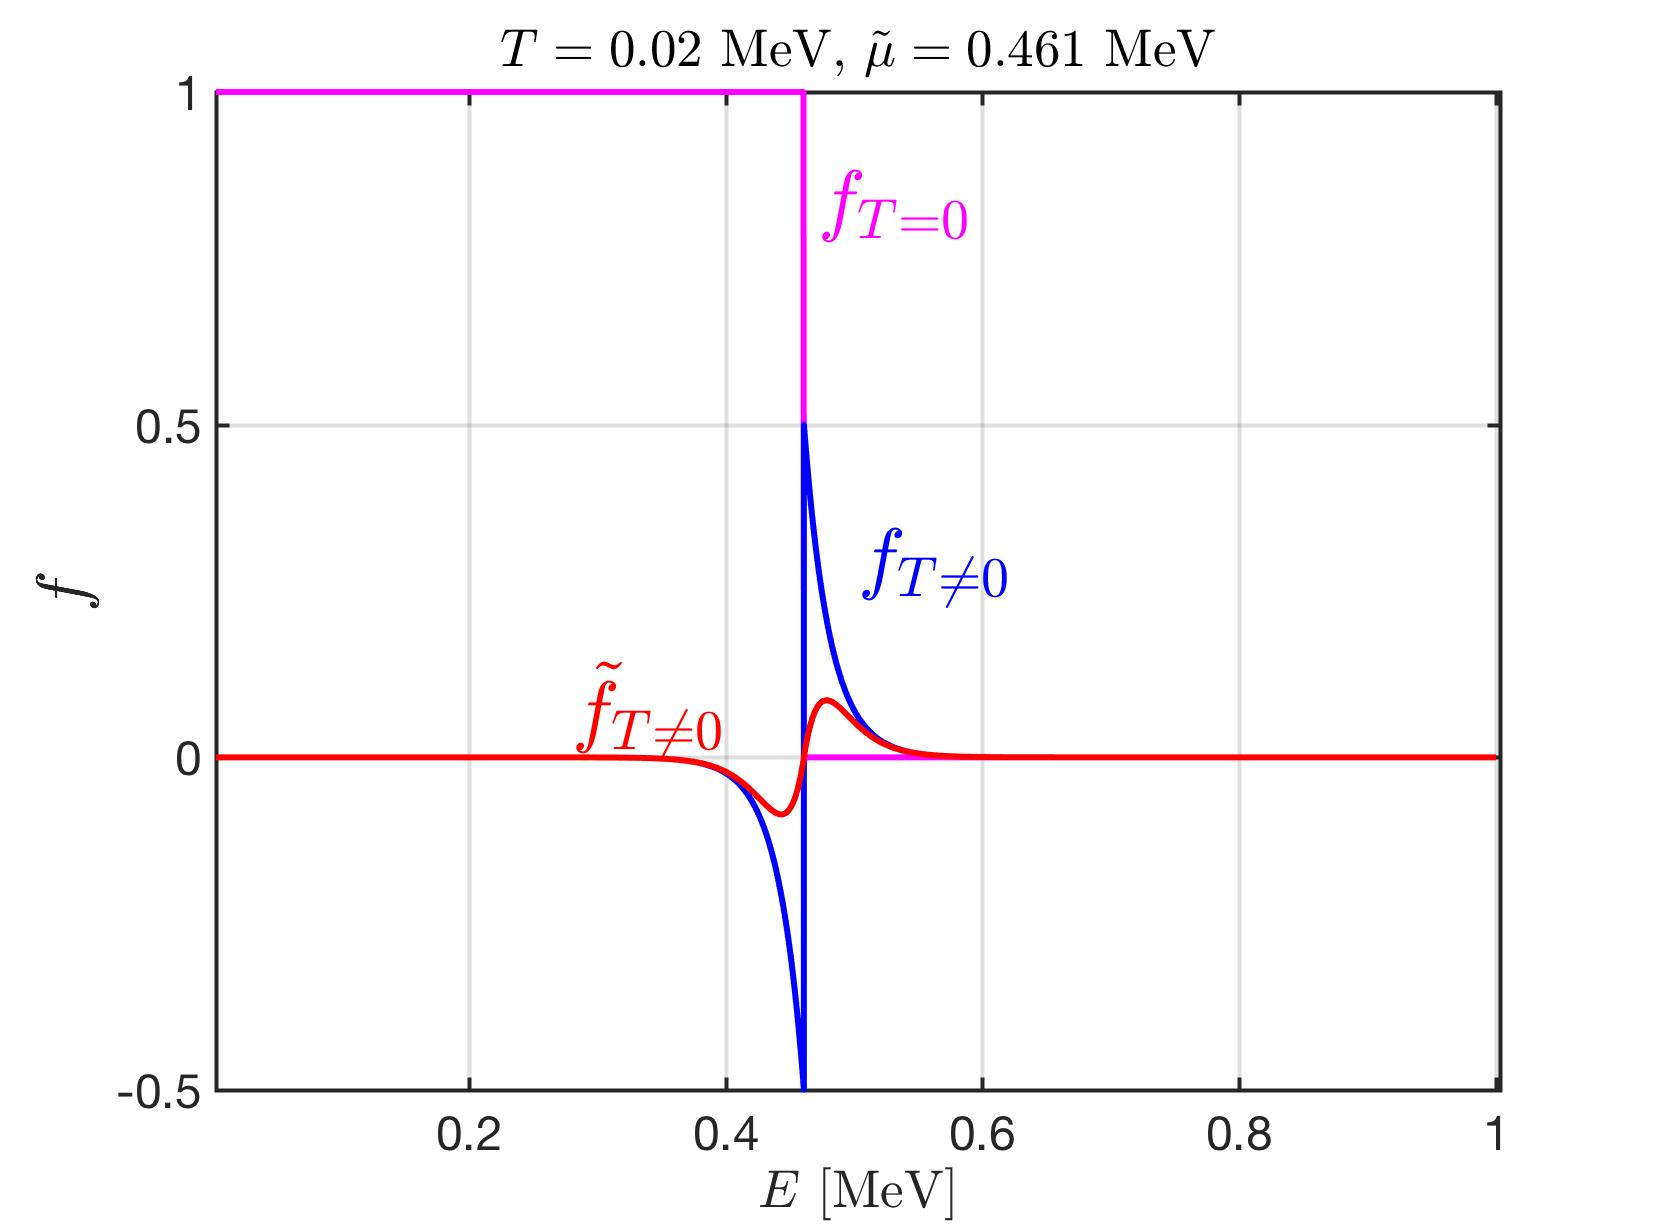
\includegraphics[width=0.5\textwidth]{./plot/FermiZeorFiniteTemperature}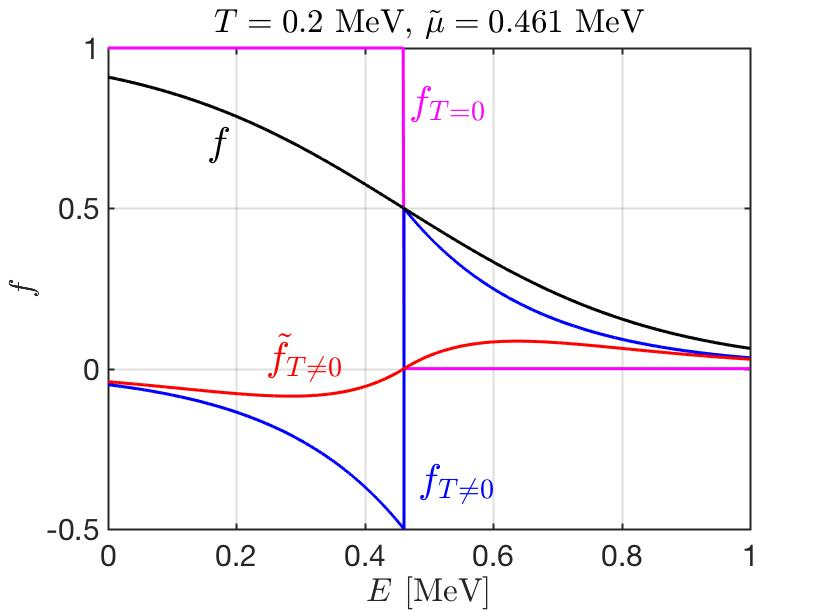
\includegraphics[width=0.5\textwidth]{./plot/FermiZeroFiniteTemperature002}
\caption{%\rev{Here I would add the full fermi distribution - to see how it is decomposed to zero temperature and finite temperature terms.}
The zero and finite temperature components of the decomposition here considered for Fermi distribution as a function of energy with chemical potential $\widetilde\mu=0.461\MeV$ at temperature $T=0.02\MeV$ and $T=0.2\MeV$. The black line represents the exact Fermi distribution. The purple line represents the zero temperature component $f_{\mathrm{T}=0}$, and blue and red lines represent the finite temperature components $f_\mathrm{T\neq0}$ and $\tilde f_\mathrm{T\neq0}$ respectively. }
\label{Fermi_Component}
\end{figure}
%%%%%%%%%%%%%%%%%%%%%%%%%%%%%%%%%%%%%%%

The Fig.~(\ref{Fermi_Component}) shows that \rev{the contributions of the two finite temperature components $f_\mathrm{T\neq0}$ and $\tilde f_\mathrm{T\neq0}$ exponentially decay with the distance from the Fermi surface $E=\tilde{\mu}$. Moreover, the splitting was chosen in such a way that the discontinuous distribution part is fully contained in $f_\mathrm{T\neq 0}$ and $\tilde{f}_\mathrm{T\neq 0}$ is a remaining smooth function of $T$. Hmmm...actually the second derivative of $\tilde{f}_\mathrm{T\neq 0}$ is discontinuous at origin, is there any other motiviation for this splitting?}  Both finite temperature contributions always have the same sign \rev{and lower the distribution for $E < \tilde{\mu}$ and increase it for $E > \tilde{\mu}$}.
%\vfill\eject


{\xred(Comments for the numerical motivation:) In contrast to the brute force approach for eliminating the $T=0$ limit from the low-temperature Fermi distribution, our analytic form of distribution offers a more numerically advantageous method for separating the finite temperature components. This is advantage arise from the behavior of: 1.) both finite temperature contributions $f_\mathrm{T\neq0}$ and $\tilde f_\mathrm{T\neq0}$ always have the same sign 2.) the exponential factor for finite temperature components provide the naturally exponentially suppresses for the large energy. In this scenario, it reduces the numerical noise when evaluate the numerical integral beyond the zero temperature approximation. Furthermore, our novel form for Fermi distribution also provide us the tool to analytically investigate the finite temperature contributions by expanding the function around the Fermi-energy surface, which is useful for addressing physics for the finite temperature approximation.}

To illustrate the advantage of our novel form of distribution can be used to address the integrals common in statistical physics especially when temperature $T\to0$, we consider for any given function $G(E-\tilde\mu/T)$, then the correspond  thermal average physical quantity $\langle G\rangle_T$ can be written as
\begin{align}
\langle G\rangle_T&\equiv\int^{\infty}_{m}\!\!dE\,G(E-\tilde\mu/T)\,f_{FD}(E-\tilde\mu/T)=\langle G\rangle_{0}+\langle G\rangle_{\delta T},
\end{align}
where the functions $\langle G\rangle_{0}$ and $\langle G\rangle_{\delta T}$ are defined as
\begin{align}
&\langle G\rangle_{0}=\int^{\infty}_{m}\!\!dE\,G(E-\tilde\mu/T)\Theta(-E+\tilde\mu/T),\\
&\langle G\rangle_{\delta T}=\int^{\infty}_{m}\!\!dE\,G(E-\tilde\mu/T)\bigg[f_\mathrm{T\neq0}(E-\tilde\mu/T)+\tilde f_\mathrm{T\neq0}(E-\tilde\mu/T)\bigg]
\end{align}
To simplify the notation, it is convenient to introduce the dimensionless variables as follows:
\begin{align}
x\equiv\left(\frac{E-\tilde\mu}{T}\right), \qquad x_0=\left(\frac{m-\tilde\mu}{T}\right),\qquad \tilde\mu>m.
\end{align}
where for the condition $T\to0$ the chemical potential $\tilde\mu$ is equal to the Fermi energy $E_F$ and we have the condition $\tilde\mu(T=0)= E_F>m$. Then the finite temperature contribution $\langle G\rangle_{\delta T}$ can be written as
\begin{align}\label{G_deltaT}
\langle G\rangle_{\delta T}&=T\int_{-|x_0|}^\infty \!\!dx\,G(x)\bigg[f_\mathrm{T\neq0}(x)+\tilde f_\mathrm{T\neq0}(x)\bigg]\notag\\
&=T\bigg[-\int^{-|x_0|}_{-\infty}\!\!dx\,G(x)\bigg(f_\mathrm{T\neq0}(x)+\tilde f_\mathrm{T\neq0}(x)\bigg)+\int_{-\infty}^{\infty}\!\!dx\,G(x)\bigg(f_\mathrm{T\neq0}(x)+\tilde f_\mathrm{T\neq0}(x)\bigg)\bigg]\notag
\\&=\langle G_1\rangle_{\delta T}+\langle G_2\rangle_{\delta T}
\end{align}
where the function $\langle G_1\rangle_{\delta T}$ and $\langle G_2\rangle_{\delta T}$ are defined by
\begin{align}
&\langle G_1\rangle_{\delta T}=-T\int^{-|x_0|}_{-\infty}\!\!dx\,G(x)\bigg(f_\mathrm{T\neq0}(x)+\tilde f_\mathrm{T\neq0}(x)\bigg)\\
&\langle G_2\rangle_{\delta T}=T\int_{-\infty}^{\infty}\!\!dx\,G(x)\bigg(f_\mathrm{T\neq0}(x)+\tilde f_\mathrm{T\neq0}(x)\bigg)
\end{align}

In general the integral of $\langle G_1\rangle_{\delta T}$ can be written as
\begin{align}
\langle G_1\rangle_{\delta T}&=-\frac{T}{2}\int^{-|x_0|}_{-\infty}\!\!dx\,G(x) e^{-|x|}\bigg(\mathrm{sgn}\left(x\right)+\tanh\left(\frac{x}{2}\right)\bigg)\notag\\
&=-\frac{T}{2}\int^{-|x_0|}_{-\infty}\!\!dx\,G(x) e^{-|x|}\bigg(-1+\tanh\left(\frac{x}{2}\right)\bigg).
\end{align}
{
\color{blue} If we change the dimensionless variables 
\begin{align}
x^\prime=\frac{1}{x}=\frac{T}{E-\tilde\mu},\qquad x_0^\prime=\frac{1}{x_0}=\frac{T}{m-\tilde\mu},
\end{align}
then the integral $\langle G_1\rangle_{\delta T}$ can be written as
\begin{align}
\langle G_1\rangle_{\delta T}&=\frac{T}{2}\int^{-|x_0^\prime|}_{0}\!\!dx^\prime\,G(1/x^\prime) e^{-|1/x^\prime|}\bigg[-1+\tanh\left(\frac{1}{2x^\prime}\right)\bigg]\\
&=\frac{T}{2}\int_{-|x_0^\prime|}^{0}\!\!dx^\prime\,G(1/x^\prime) e^{-|1/x^\prime|}\bigg[1-\tanh\left(\frac{1}{2x^\prime}\right)\bigg]
\end{align}
}

 Given any regular function $G(x)$, there is no singularity in the integral. Hence we propose that the integral for finite temperature contribution $\langle G_1\rangle_{\delta T}$ can be written as
\begin{align}\label{finite expansion}
\langle G_1\rangle_{\delta T}=\sum_{n}c_nT^n,
\end{align}
where $c_n$ represents the coefficients used to expand the function in terms of temperature.


%By employing our decomposition form, we propose that the integral for finite temperature contribution $\langle G\rangle_{\delta T}$ in general can be written as
%\begin{align}\label{finite expansion}
%\langle G\rangle_{\delta T}=\sum_{n}c_nT^n,
%\end{align}
%where $c_n$ represents the coefficients used to expand the function in terms of temperature. In this scenario, our novel Fermi distribution can provide the tool to study any physical quantity when temperature approach to zero, and facilitate the connection between the study of finite temperature system to zero temperature limit smoothly. 

%In following we will demonstrate that for any general function in the zero-temperature limit, we can always write the integral into Eq.~(\ref{finite expansion}). 
On the other hand, the function $\langle G_2\rangle_{\delta T}$ can be written as 
\begin{align}
\langle G_2\rangle_{\delta T}=\frac{T}{2}\int^{\infty}_{-\infty}\!\!dx\,G(x) e^{-|x|}\bigg(\mathrm{sgn}\left(x\right)+\tanh\left(\frac{x}{2}\right)\bigg).
\end{align}
In general, for any function $G(x)$ we can use the Laguerre polynomials $L_n(x)$ as a basis to expand it. We have
\begin{align}
G(x)=\sum_{n}k_nL_n(x),\qquad k_n=\int_0^\infty\!\!dx G(x)L_n(x)e^{-x},\qquad n=0,1,2,\cdots
\end{align}
where $k_n$ represents the expansion coefficients. In this case, the finite temperature contribution $\langle G_2\rangle_{\delta T}$ can be written as
\begin{align}
&\langle G_2\rangle_{\delta T}\!=\!\frac{T}{2}\sum_n k_n\!\!\int^{\infty}_{-\infty}\!\!\!\!dx\,L_n(x) e^{-|x|}\bigg(\mathrm{sgn}\left(x\right)+\tanh\left(\frac{x}{2}\right)\!\!\bigg)\!\!=\frac{T}{2}\sum_n k_n\bigg(a_n+b_n\bigg)\\
&a_n=\int^{\infty}_{-\infty}\!\!\!\!dx\,L_n(x) e^{-|x|}\mathrm{sgn}\left(x\right),\qquad b_n=\int^{\infty}_{-\infty}\!\!\!\!dx\,L_n(x) e^{-|x|}\tanh\left(\frac{x}{2}\right)
\end{align}

Given different value of $n=0,1,2,3\cdots$, the integral can be evaluated numerically. In Table.~\ref{coeff_table} we evaluate the coefficient $a_n$ and $b_n$ numerically for $n=1,2,3,4$ as an example.  %~~~~~~~~~~~~~~~~~~~~~~~~~~~~~~~~~~~~~~~~~~~~~~~~~~~~~~~~~~~~~~~~~~~~~~~~~~~~~~~~~~~~~~~~~
\begin{table}%[b]
\centering
\begin{tabular}{c| c| c}
\hline\hline
$n$ &$a_n$ & $b_n$ \\
\hline
$0$ & $0$ & $0$\\ 
\hline
$1$ & $-2$ & $(6-\pi^2)/3$\\
\hline
$2$ & $-4$& $2(6-\pi^2)/3$\\
\hline
 $3$ & $-8$&$(1140-180\pi^2-7\pi^4)/180$\\
\hline
$4$ & $-16$ & $(720-60\pi^2-7\pi^4)/45$\\
\hline\hline
\end{tabular}
\caption{The coefficient $a_n$ and $b_n$ for $n=1,2,3,4$ as example.}
\label{coeff_table} 
\end{table}

%~~~~~~~~~~~~~~~~~~~~~~~~~~~~~~~~~~~~~~~~~~~~~~~~~~~~~~ 


%%%%%%%%%%%%%%%%%%%%%%%%%%%%%%%%%%%%%%%
\section{Results and Discussion}
\label{sec12}
In this work, we introduce a novel form of the Fermi distribution Eq.~(\ref{NFF1}) that separates the Fermi gas into zero and finite temperature components analytically. This is the first time in literature that has clean separation of the zero and finite temperature components. Unlike the traditional brutal approach to eliminating the $T=0$ limit from the low-temperature Fermi distribution, our novel form of the Fermi distribution for finite temperature component has several numerical advantages in computation. 

The Fermi distribution Eq.~(\ref{NFF1}) provides us the tool to study or examine the effects and characteristics of finite temperature components separately. The mathematical form of the finite temperature components is well-suited for numerical calculations and can be used to address the integrals common in statistical physics. This is because the finite temperature components are naturally exponentially suppressed while also preserving the sign of all corrections making the formulation easier to numerically integrate and reduce the numerical noise, see Fig.~\ref{Fermi_Component}. In addition, our approach also allows for analytical exploration of the finite temperature contributions by expanding the function around the Fermi-energy surface.

To illustrate the numerical benefits, we examine the magnetization of electron-positron gas in a uniform magnetic filed as an example. Fig.~\ref{M_Checking001} shows that our novel form of Fermi distribution improves convergence of the numerical calculation of Landau levels. Instead of summing over a large number of terms, our approach  requires only a few additional terms in the Landau level summation to obtain the stable magnetization. This results imply that our analytic form of Fermi function exhibits rapid convergence and therefore improves the computational efficiency significantly.



%%%%%%%%%%%%%%%%%%%%%%%%%%%%%%%%%%%%%%%


% Martin - Highlight the method can be used to address the integrals common in stastistical physics.
% Johann - First time we separate cleanly the hot and cold components. This therefore could be very useful for studying interacting systems where the mathematics becomes intractible quickly. The properties near to the Fermi surface are clearly isolated and most of the interactions occur near the Fermi surface.
% Cold matter cannot form pairs, but finite temperature systems can because of the deformation of the step function. Particle-antiparticle hope pairs behavior is isolated. May have applications to superconducting systems. Allowing for the exploration of interacting systems at the Fermi surface.
% Reference to superconducting neutron stars.
% Andrew - This allows us to analyze the finite temperature elements as a distinct model.
% Cheng Tao - This novel form is numerically friendly as the finite temperature components are naturally exponentially suppresses while also preserving the sign of all corrections making the formulation easier to numerically integrate.

%%%%%%%%%%%%%%%%%%%%%%%%%%%%%%%%%%%%%%%
%\section{Appendix}
%\label{Append}
%%%%%%%%%%%%%%%%%%%%%%%%%%%%%%%%%%%%%%%
%%%%%%%%%%%%%%%%%%%%%%%%%%%%%%%%%%%%%%%%%%%
%%%%%%%%%%%%%%%%%%%%%%%%%%%%%%%%%%%%%%%
\backmatter

\bmhead{Acknowledgments}
We thank Gordon Baym and John W. Clark for their encouragement to publish this result.

%%%%%%%%%%%%%%%%%%%%%%%%%%%%%%%%%%%%%%%
\bibliography{novel-fermi-function-refs}
%% if required, the content of .bbl file can be included here once bbl is generated
%%\input sn-article.bbl
\end{document}
